\documentclass[a4paper,12pt]{article}
\usepackage[utf8]{inputenc} % input encdoding = written input text to latex
\usepackage[T1]{fontenc} % encoding = compiled latex to output font
\usepackage{natbib}% support (author-year, numbered, etc.), also improved compatibility with bib managing
\usepackage{microtype} % microtypography is the art of enhancing the appearance of a document while exhibiting the minimum degree of visual obtrubsion
\usepackage{newpxtext,newpxmath} % vectorial palatino-like font with support for math, siunitx, mchem, etc. It is also darker than standard latex font
\usepackage[left=2cm,right=2cm,top=3cm,bottom=3cm,headheight=15pt]{geometry} % adjust layout - borders
\usepackage{emptypage} % avoid headers and footers on white pages.
\usepackage[parfill]{parskip} % pararaph layout (white vertical space, last paragraph line with minimum space, etc.)
\usepackage{makecell}
\usepackage{multirow} % macros for tabular env. etc. (multirow cells, ...)
\usepackage{tabularx,ragged2e} % extention of tabular with column X, which automatically adjusts width etc
\usepackage{float} % improved management (H, ...) for floating objects
\usepackage{bm} % bold in math mode (e.g., vector fields)
\usepackage{graphicx} % extention of the graphics package, including key-value interface for the includegraphics command 
\usepackage{caption}
\usepackage{subcaption} % for formatting captions and subcaptions
\usepackage{booktabs} % for professional looking tables
\usepackage[version=4]{mhchem} % chemical formulas
\usepackage{amsfonts}
\usepackage{pdflscape}
\usepackage{amssymb} % extended set of fonts and symbols for mathematics
\usepackage{amsmath} % improve structure and output of documents that contain mathematics
\usepackage{mathtools} % based on amsmath, it improves looking and provide new capabilities and options (numbering, format, etc.)
\usepackage{pdfpages}
\usepackage{textcomp} % extended set of fonts and symbols
\usepackage[toc,page]{appendix} % allows appendices
\usepackage{epigraph}
\setlength\epigraphwidth{0.7\textwidth}
\setlength\epigraphrule{0pt} % allow epighaphs and provide various handles to tweak the appearance
\usepackage{listings} % include code
\usepackage{siunitx} % standard input of units and numbers (SI, si, num, etc.)
\sisetup{separate-uncertainty, multi-part-units=single, detect-family, detect-weight, range-units=single}
\usepackage[compact]{titlesec} % managing titles, headers, etc. Compact reduces spaces above and below the titles
\usepackage{fancyhdr}
\usepackage{hyperref}
\usepackage{xcolor}
\hypersetup{colorlinks, linkcolor=[rgb]{0.1,0.2,0.7}, citecolor=[RGB]{120,0,0}, urlcolor=[rgb]{0.1,0.2,0.7}}
\title{Noble ERT updates}
\author{}
\date{28 Apr 2020}
\begin{document}
\setcounter{secnumdepth}{0} % avoid section numbering
\newcommand{\myseparator}{\noindent\makebox[\linewidth]{\resizebox{0.5\linewidth}{1pt}{$\bullet$}}\bigskip}
\newcommand{\subwidth}{0.48}
\graphicspath{{./../}{./../figures/}{./figures/}}
%\maketitle

%\begin{figure}[H]
%\centering
%\begin{subfigure}{\textwidth}
%\includegraphics[width=\textwidth]{}
%\end{subfigure}
%\end{figure}

\section{Briefly data acquisition and inversion}
The ERT acquisitions started October 25 2019, this report is up to 28 April 2020.
I'm now running the ERT once a day.
We started with a DD2 array, till Nov 18, first 4 datasets.
Then two types of gradient array were used, which limited the power usage while targeting the root zone with fewer but higher-quality data.
As for the DD2, gradient arrays were optimized for the 8-channel resistivity meter, average number of data points per injection about 7.
Acquisition parameters were: stack \num{4}, injection time \SI{250}{\milli\second}.
Data were filtered considering reciprocity (\SI{5}{\percent}) and staking (\SI{5}{\percent}); as expected, contact resistances were always very good.
Overall, data quality is very good.
In particular, since the last gradient array was used (20 March) no data point was discharged and all data points were matched by the inversion.
Timelapse inversions were performed, both models and regularization are shared between times to constrain the resistivity changes and the smoothing variability.
Data are plotted based on the actual coverage for the transparency, this is the reason for the differences between the ERT sections of different array types.

\section{Results}
There are 10 crop plots (C01 to C10) and 11 spaces (bare soil) diving them (S01 to S11).
In the growing season, the plant plots have becoming more resistive than the spaces between them.
Here are two ert sections, one from the winter and a more recent one in growing season.

\begin{figure}[H]
\centering
\begin{subfigure}{\textwidth}
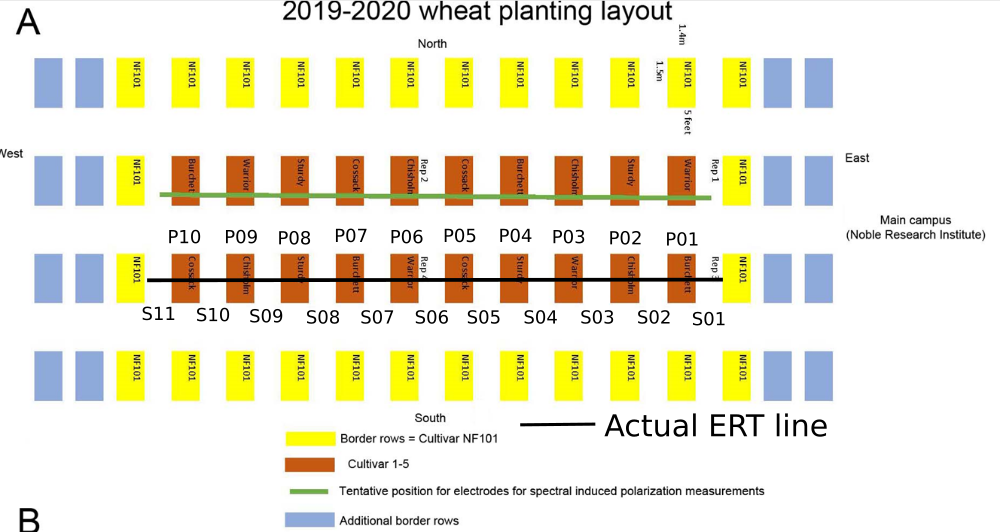
\includegraphics[width=\textwidth]{plots.png}
\end{subfigure}
\end{figure}

\begin{figure}[H]
\centering
\begin{subfigure}{\textwidth}
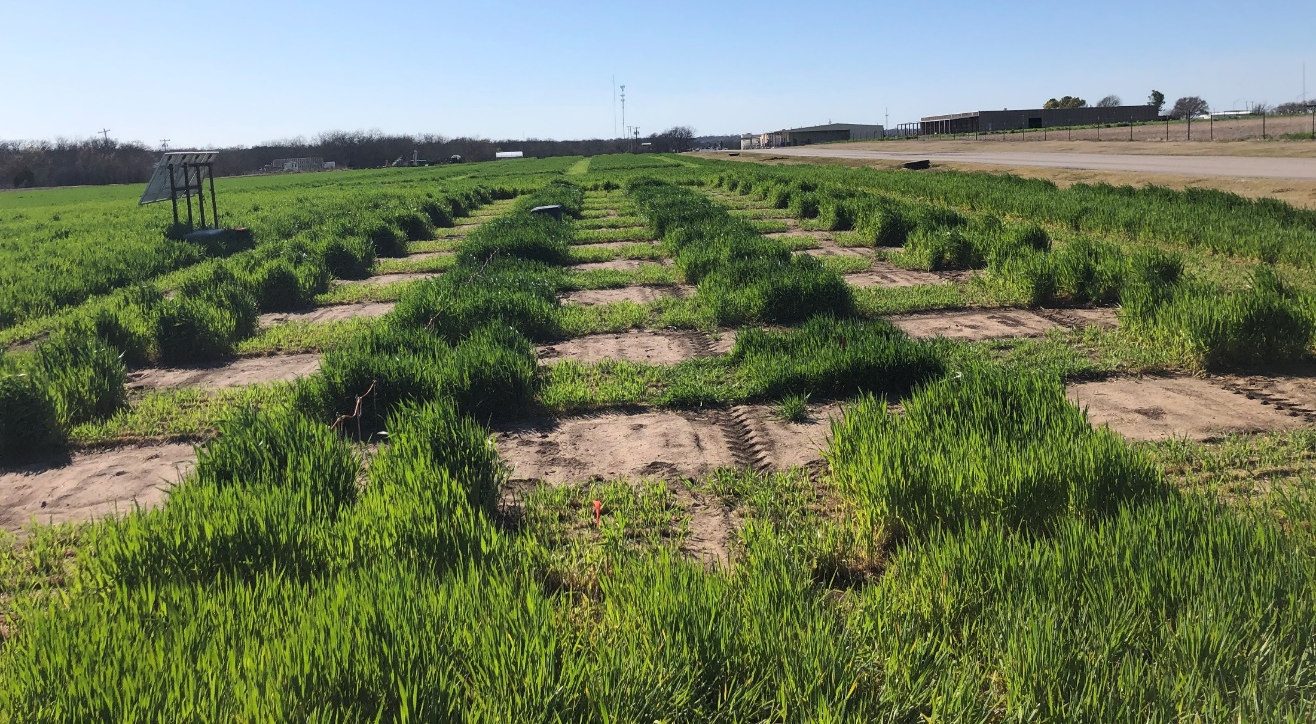
\includegraphics[width=\textwidth]{picture_plots.png}
\end{subfigure}
\end{figure}

\begin{figure}[p]
\centering
\begin{subfigure}{\textwidth}
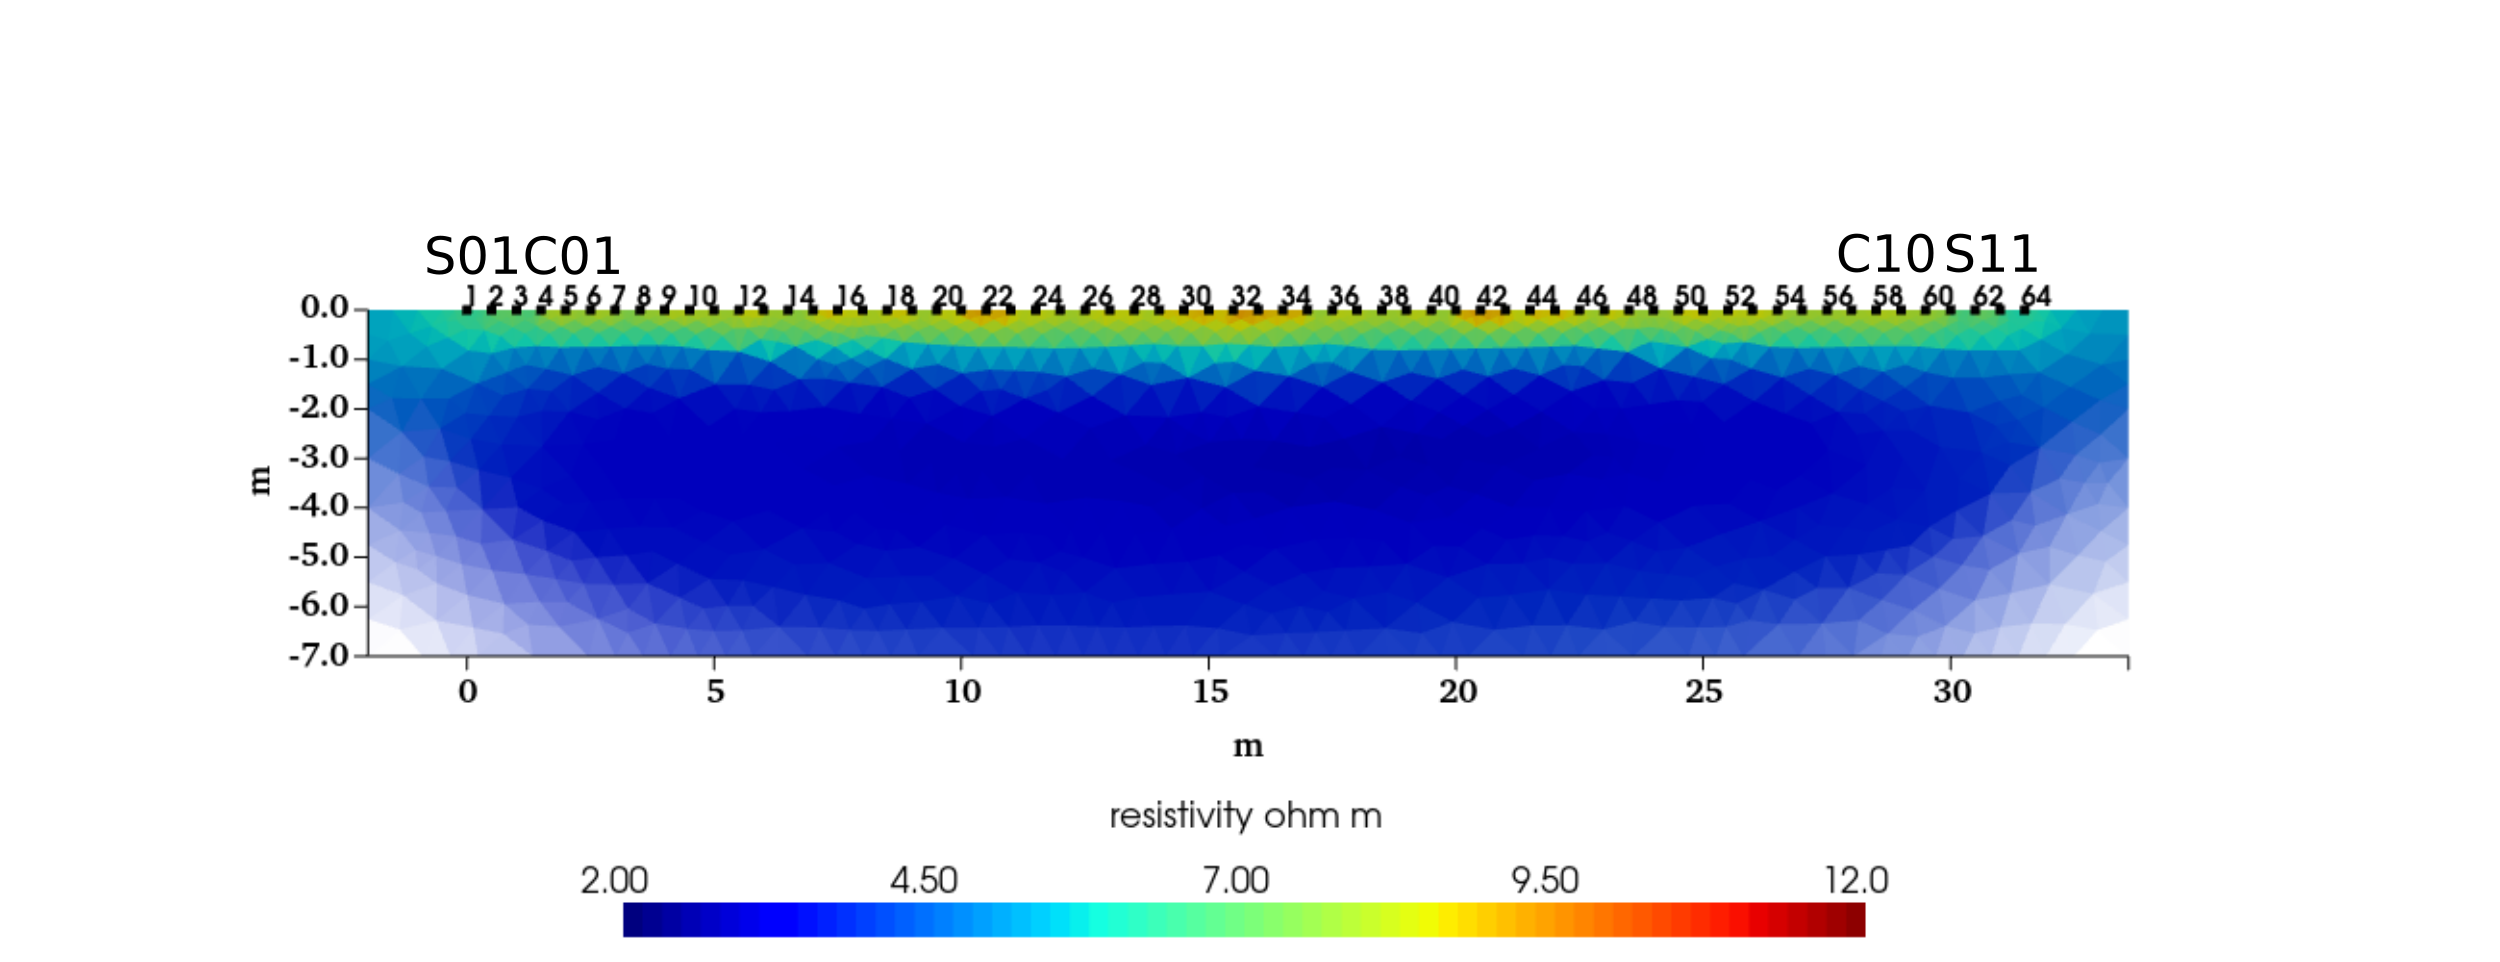
\includegraphics[width=\textwidth]{October.png}
\end{subfigure}
\caption{October 25}
\end{figure}

\begin{figure}[p]
\centering
\begin{subfigure}{\textwidth}
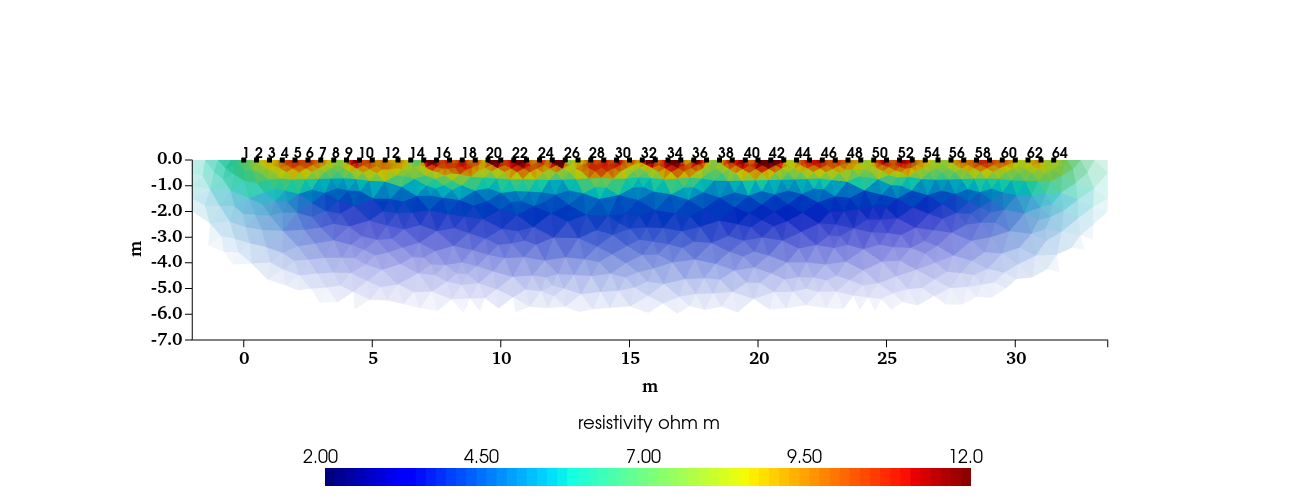
\includegraphics[width=\textwidth]{April06.png}
\end{subfigure}
\caption{April 6}
\end{figure}

\begin{figure}[p]
\centering
\begin{subfigure}{\textwidth}
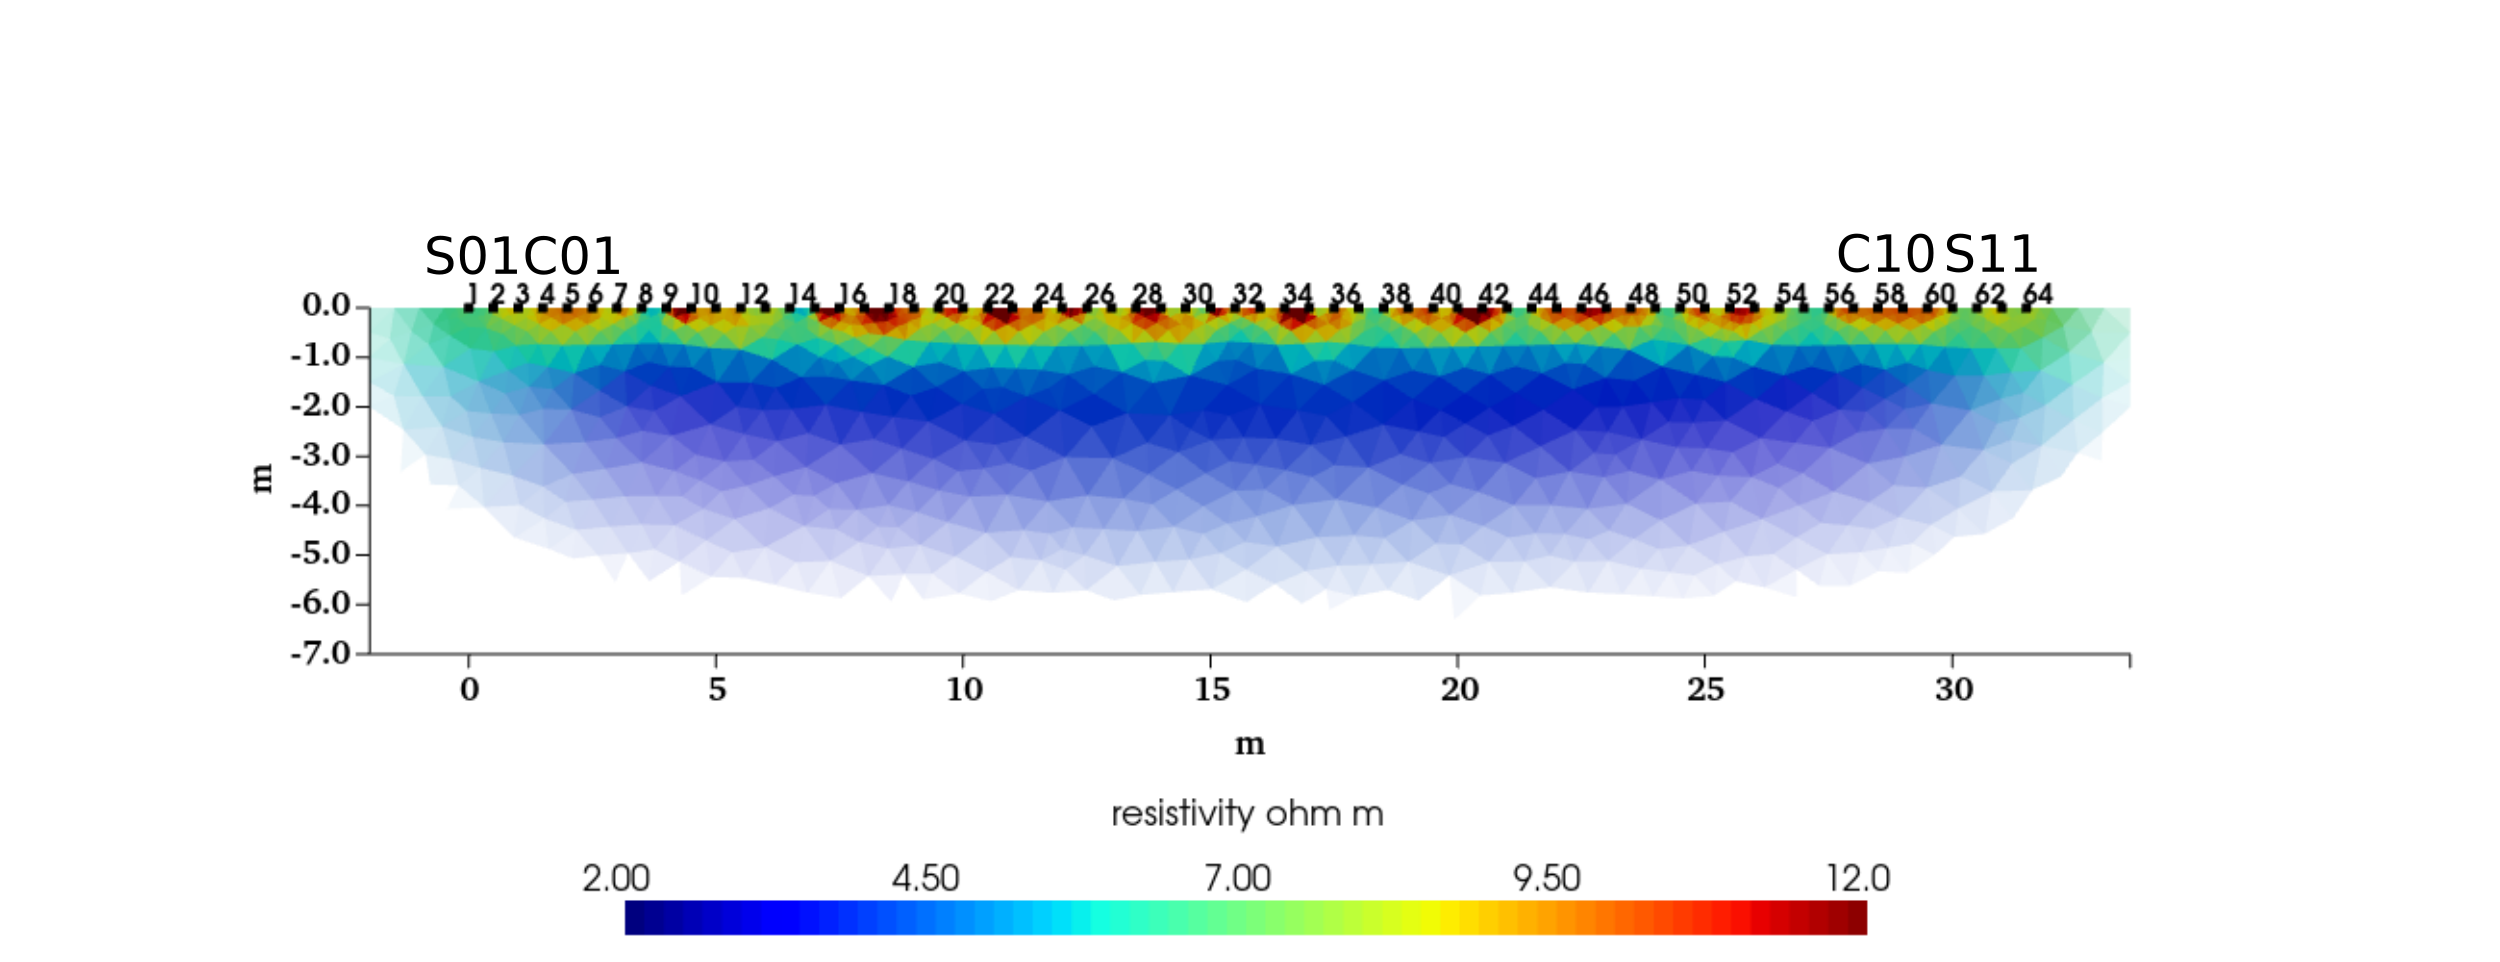
\includegraphics[width=\textwidth]{April26.png}
\end{subfigure}
\caption{April 26}
\end{figure}

\section{Resistivity}
As the RWU effect on the resistivity is evident, I extracted to resistivity average for each of the crop and space plots.
Each of the 10 crop plots is \SI{1.4}{\meter} width; while the spaces are \SI{1.5}{\meter} width.
The depth of analysis was \SI{80}{\centi\meter}, based on the ERT imaging of RWU depth.
For example, C01 goes from \SI{1.5}{\meter} to \SI{2.9}{\meter}, and from the soil surface to \SI{80}{\centi\meter} depth.
I plotted these 21 averages over time to highlight how the difference between crop plots and space plots changed with the changes in root activity (growing season).

Plant plots are in general more resistive, but this has been becoming increasingly more evident in the last few weeks.
The lines, representing the averages, are diverging.

\begin{figure}[H]
\centering
\begin{subfigure}{\textwidth}
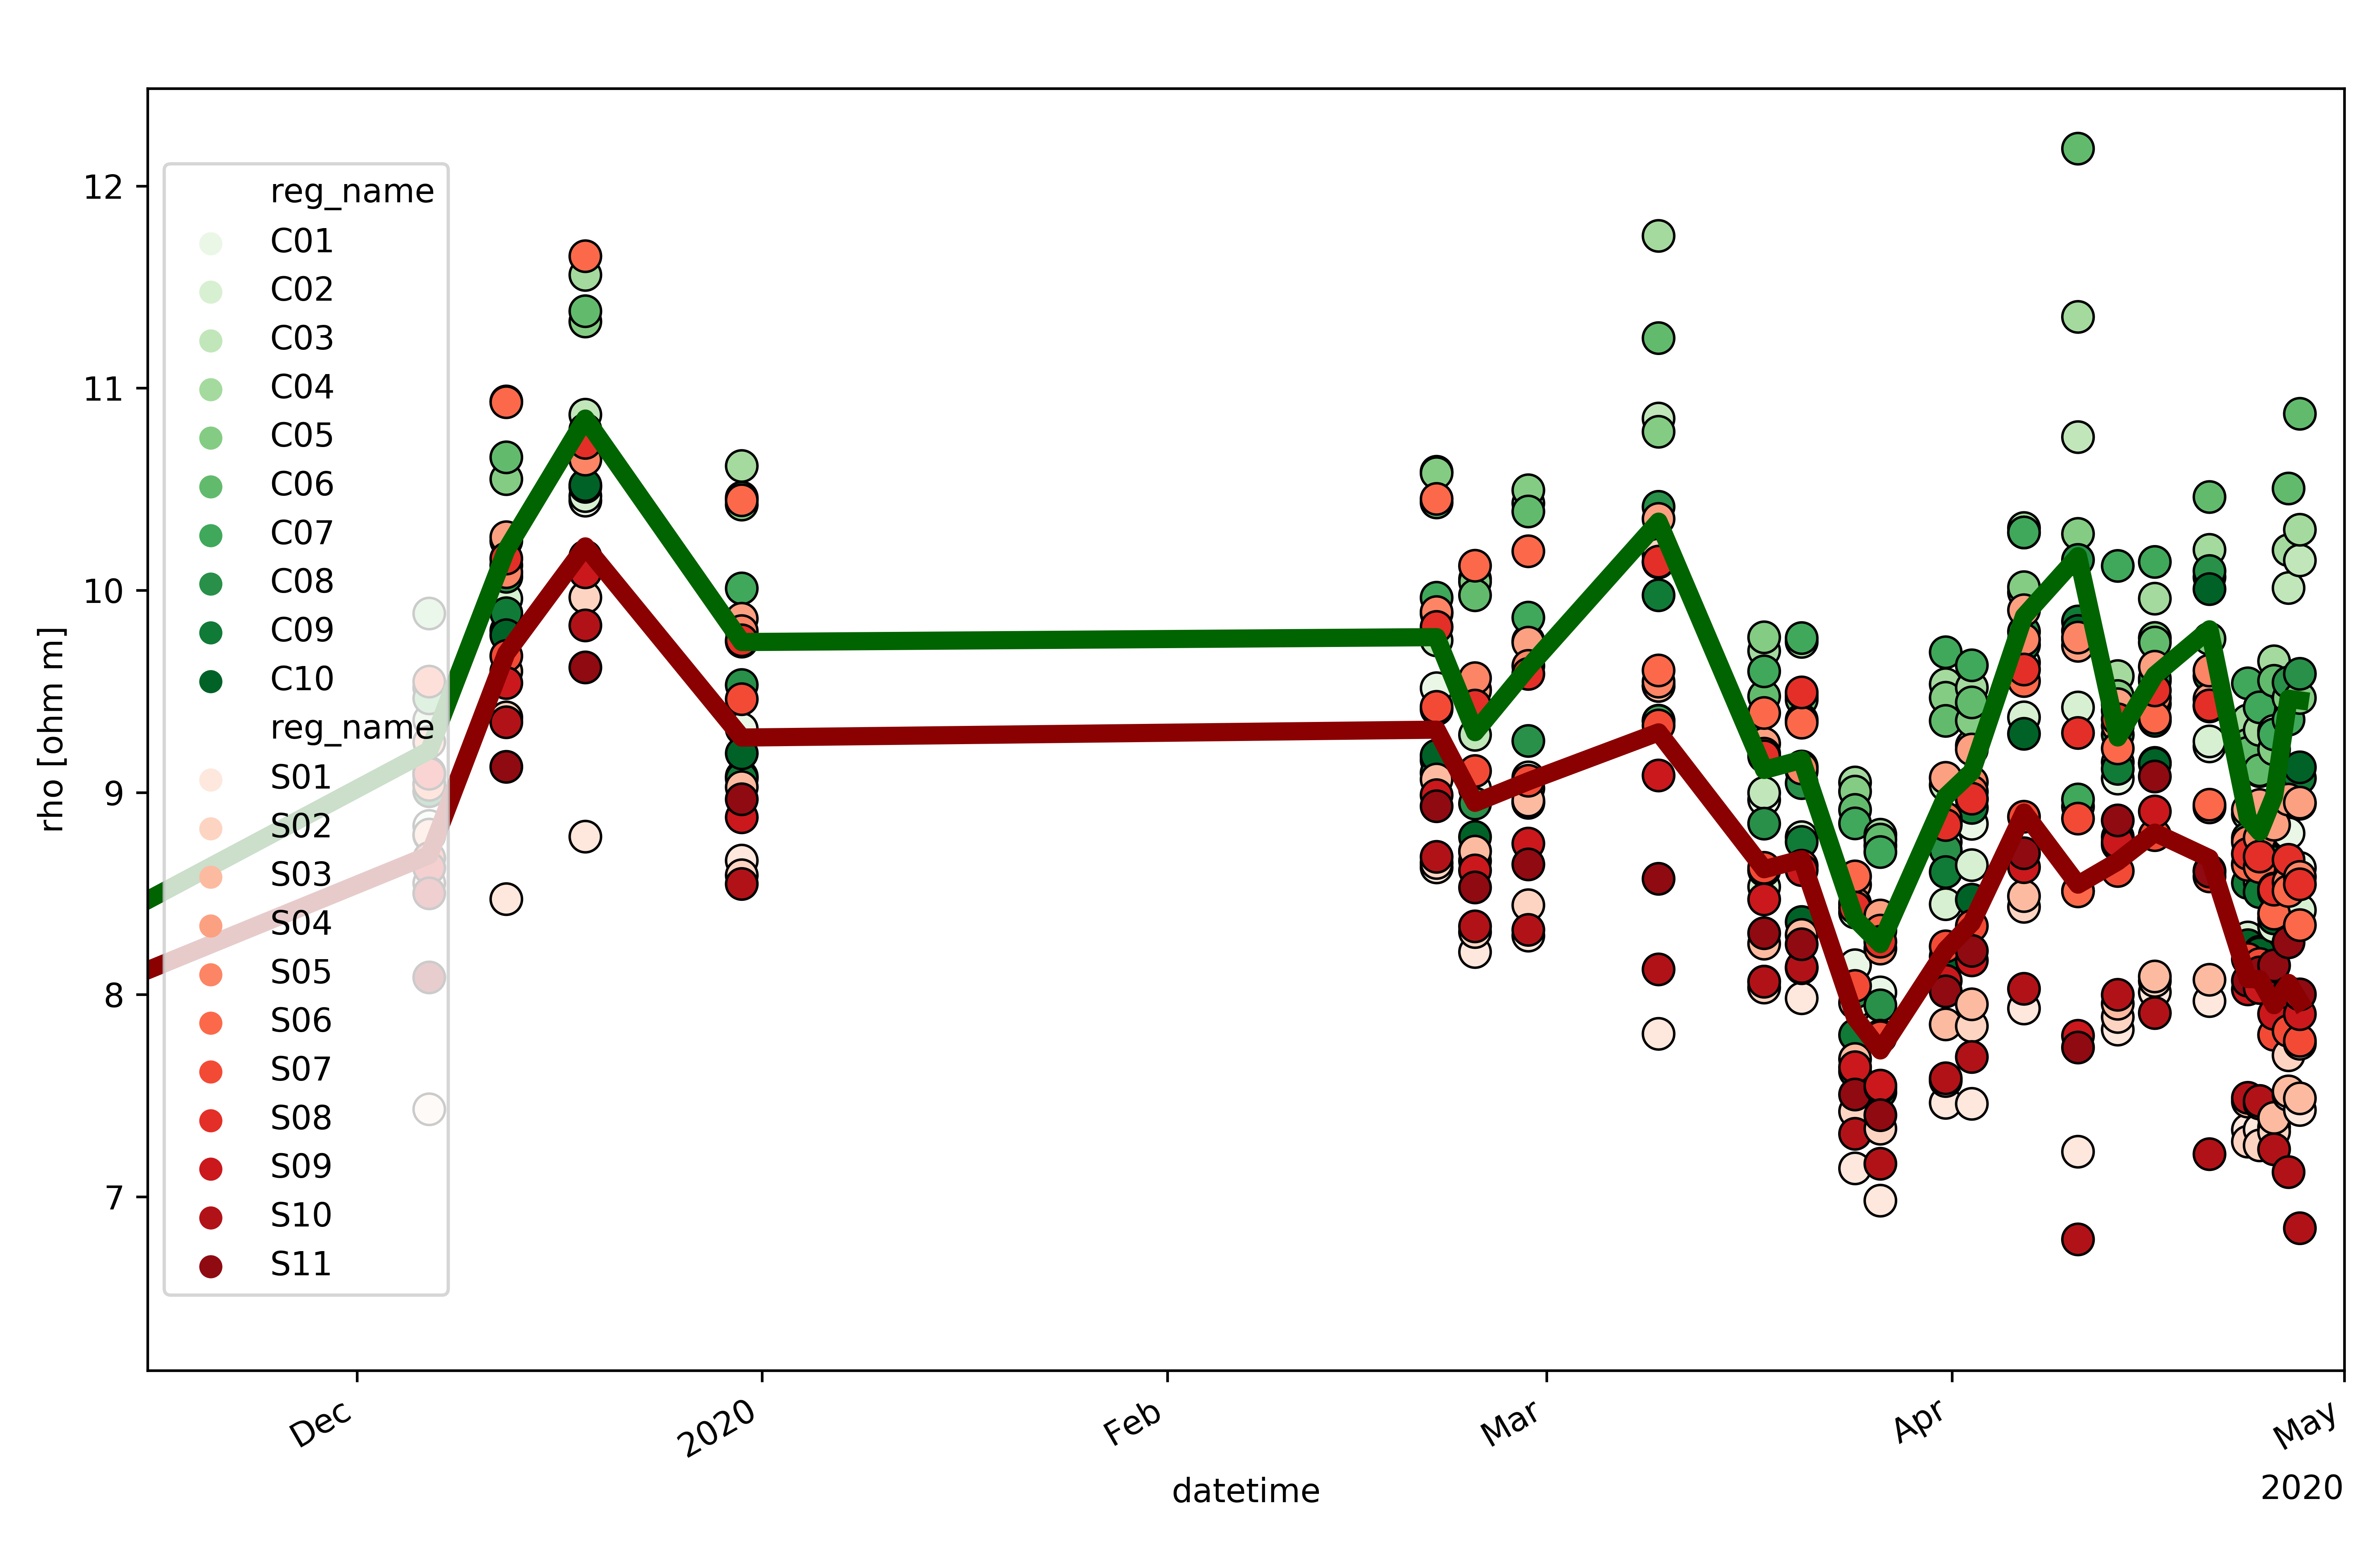
\includegraphics[width=\textwidth]{plot_analysis.png}
\end{subfigure}
\caption{Average resistivities over time for plant and space plots.
In brown/red the space plots, in green the plant plots.
The lines are the group average, to highlight the general effect of the plants on the resistivity.
Differences between crop plots are expected due to the different cultivars, as already visible on the ERT sections.}
Differences between space plots could also be related to the different cultivars as the later influence form the cultivars on the space plot is quite evident on the ERT sections.
The RWU influences on the space plots also reduce the differences between crop and space plots (i.e., the two lines would diverge more without later RWU).
This can be further investigated and it is becoming more evident with increasing RWU impact.
Finally, it may be highlighted that the two lines diverge when the resistivity increases (dry period) and converge when the resistivity decreases (homogeneous rain and associated possible water diffusion).
This didn't occur in December thoush, because the RWU played had a minor effect in that early period.
\end{figure}

\section{Resistivity and Sensors}

The data logger is a EM60G.
There are 6 sensors installed: 4 5TE (moisture, temperature, and EC) and 2 TEROS 21 (water potential and temperature).
The two types of sensors were installed in two close wells (about \SI{50}{\centi\meter} apart) that are about the center of the ERT line (\SI{15}{m} along the line, about \SI{1}{\meter} away from the line).
The 4 5TE sensors were installed at a depth of \num{18}, \num{36}, \num{53}, and \num{71} \si{\centi\meter}.
The 2 TEROS 21 were installed at a depth of \num{18} and \num{36} \si{\centi\meter}, matching the tow shallower 5TE sensors.

We can compare resistivity and data from the sensors.
For this, I focused on the resistivity changes with depth; I ignored the differences between crop and space plots, taking the entire average from \num{10} to \num{20} \si{\meter} along the ERT section.
While this allowed more data points for the averages, other solutions are possible to better account for the fact that the soil sensors are positioned on a crop plot.
I chose 5 depth intervals: \num{0} to \num{25}, \num{25} to \num{50}, \num{50} to \num{75}, \num{75} to {100}, and \num{100} to \num{150} \si{\centi\meter}.

\begin{figure}[H]
\centering
\begin{subfigure}{\textwidth}
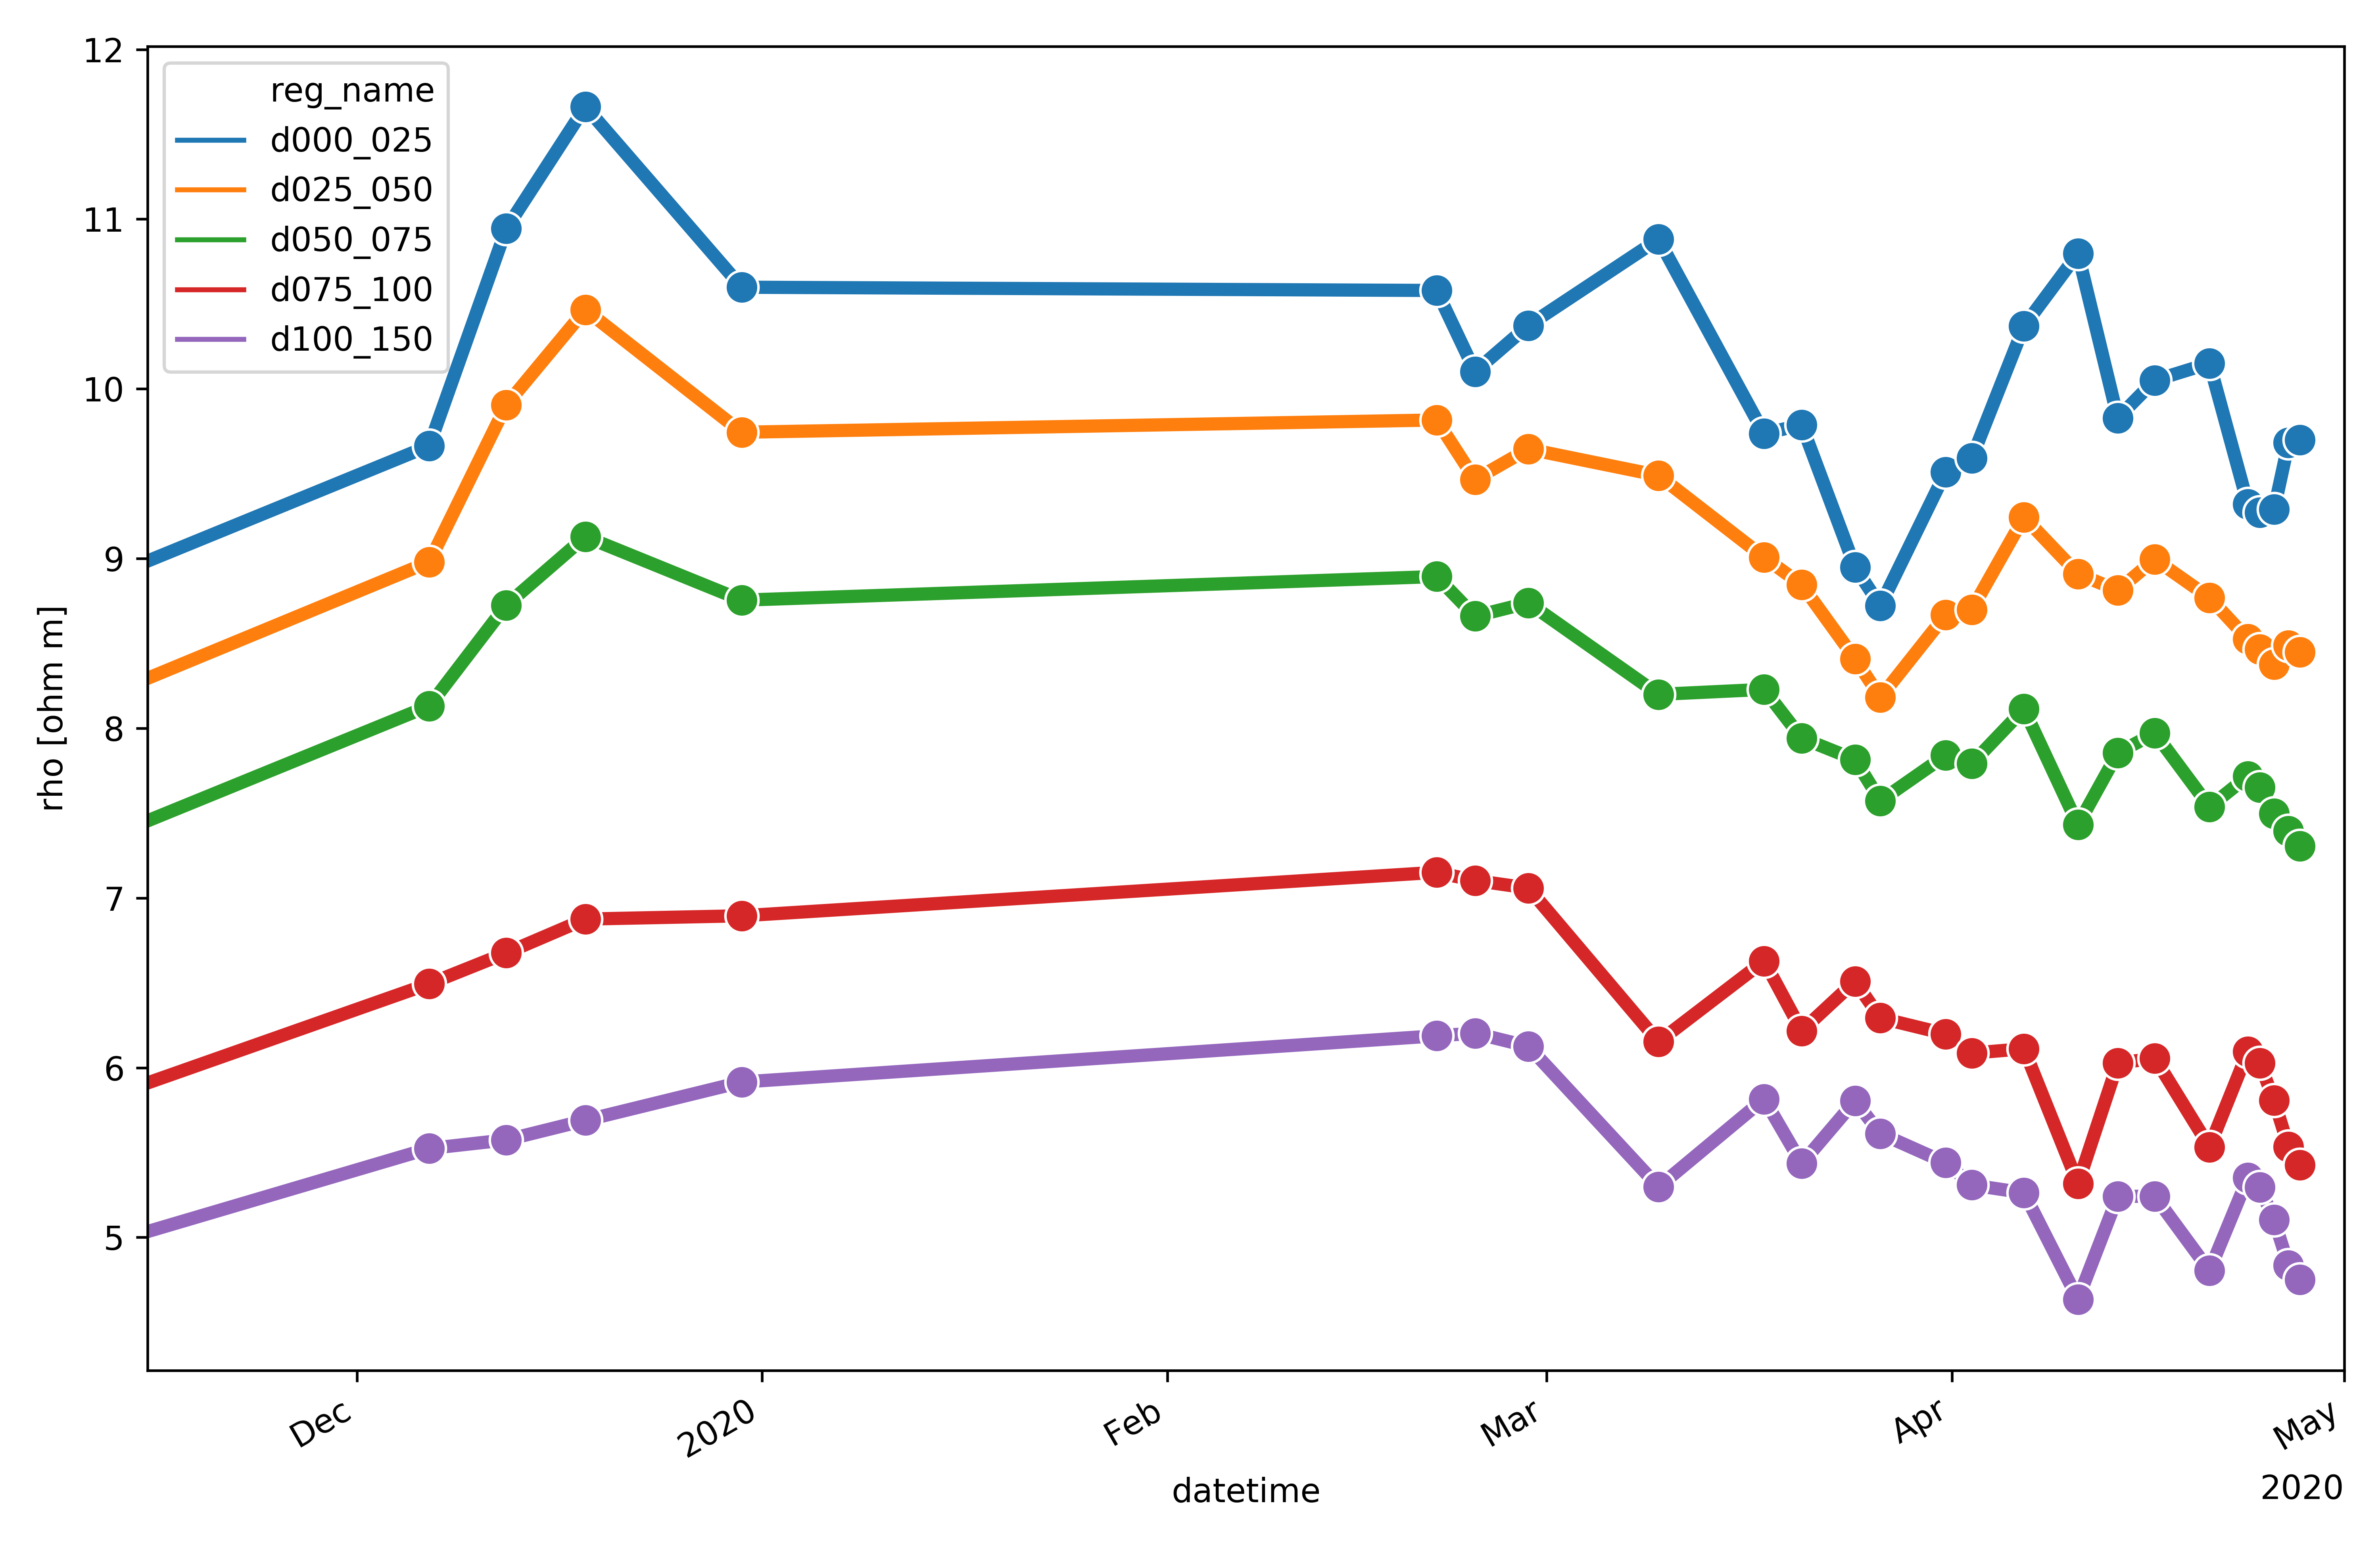
\includegraphics[width=\textwidth]{depth_analysis.png}
\end{subfigure}
\caption{Average resistivities over time for 5 different depth intervals.
The resistivity decreases with the depth.}
\end{figure}

Putting together soil sensors and ERT we can see that below \SI{80}{\centi\meter} there were limited changes in water content, the deepest sensor being at \SI{71}{\centi\meter}.
Already at \SI{53}{\centi\meter} (green line water content) there were limited changes. 
Unfortunately, we only have data from the soil sensor for a short period, without recent data to compare with the more dense ERT timelapse.
Temperature data seem very reliable, with very similar values between teros and 5TE sensors at the two common depths.

The water potentials are small (meaning not very negative) and do not respond significantly to the rain events and dry periods.
Likely to water contents are too high and to induce water suction (as discussed during the Meter webinar).
We may see more significant water suctions in the next few weeks.

\begin{figure}[H]
\centering
\begin{subfigure}{\textwidth}
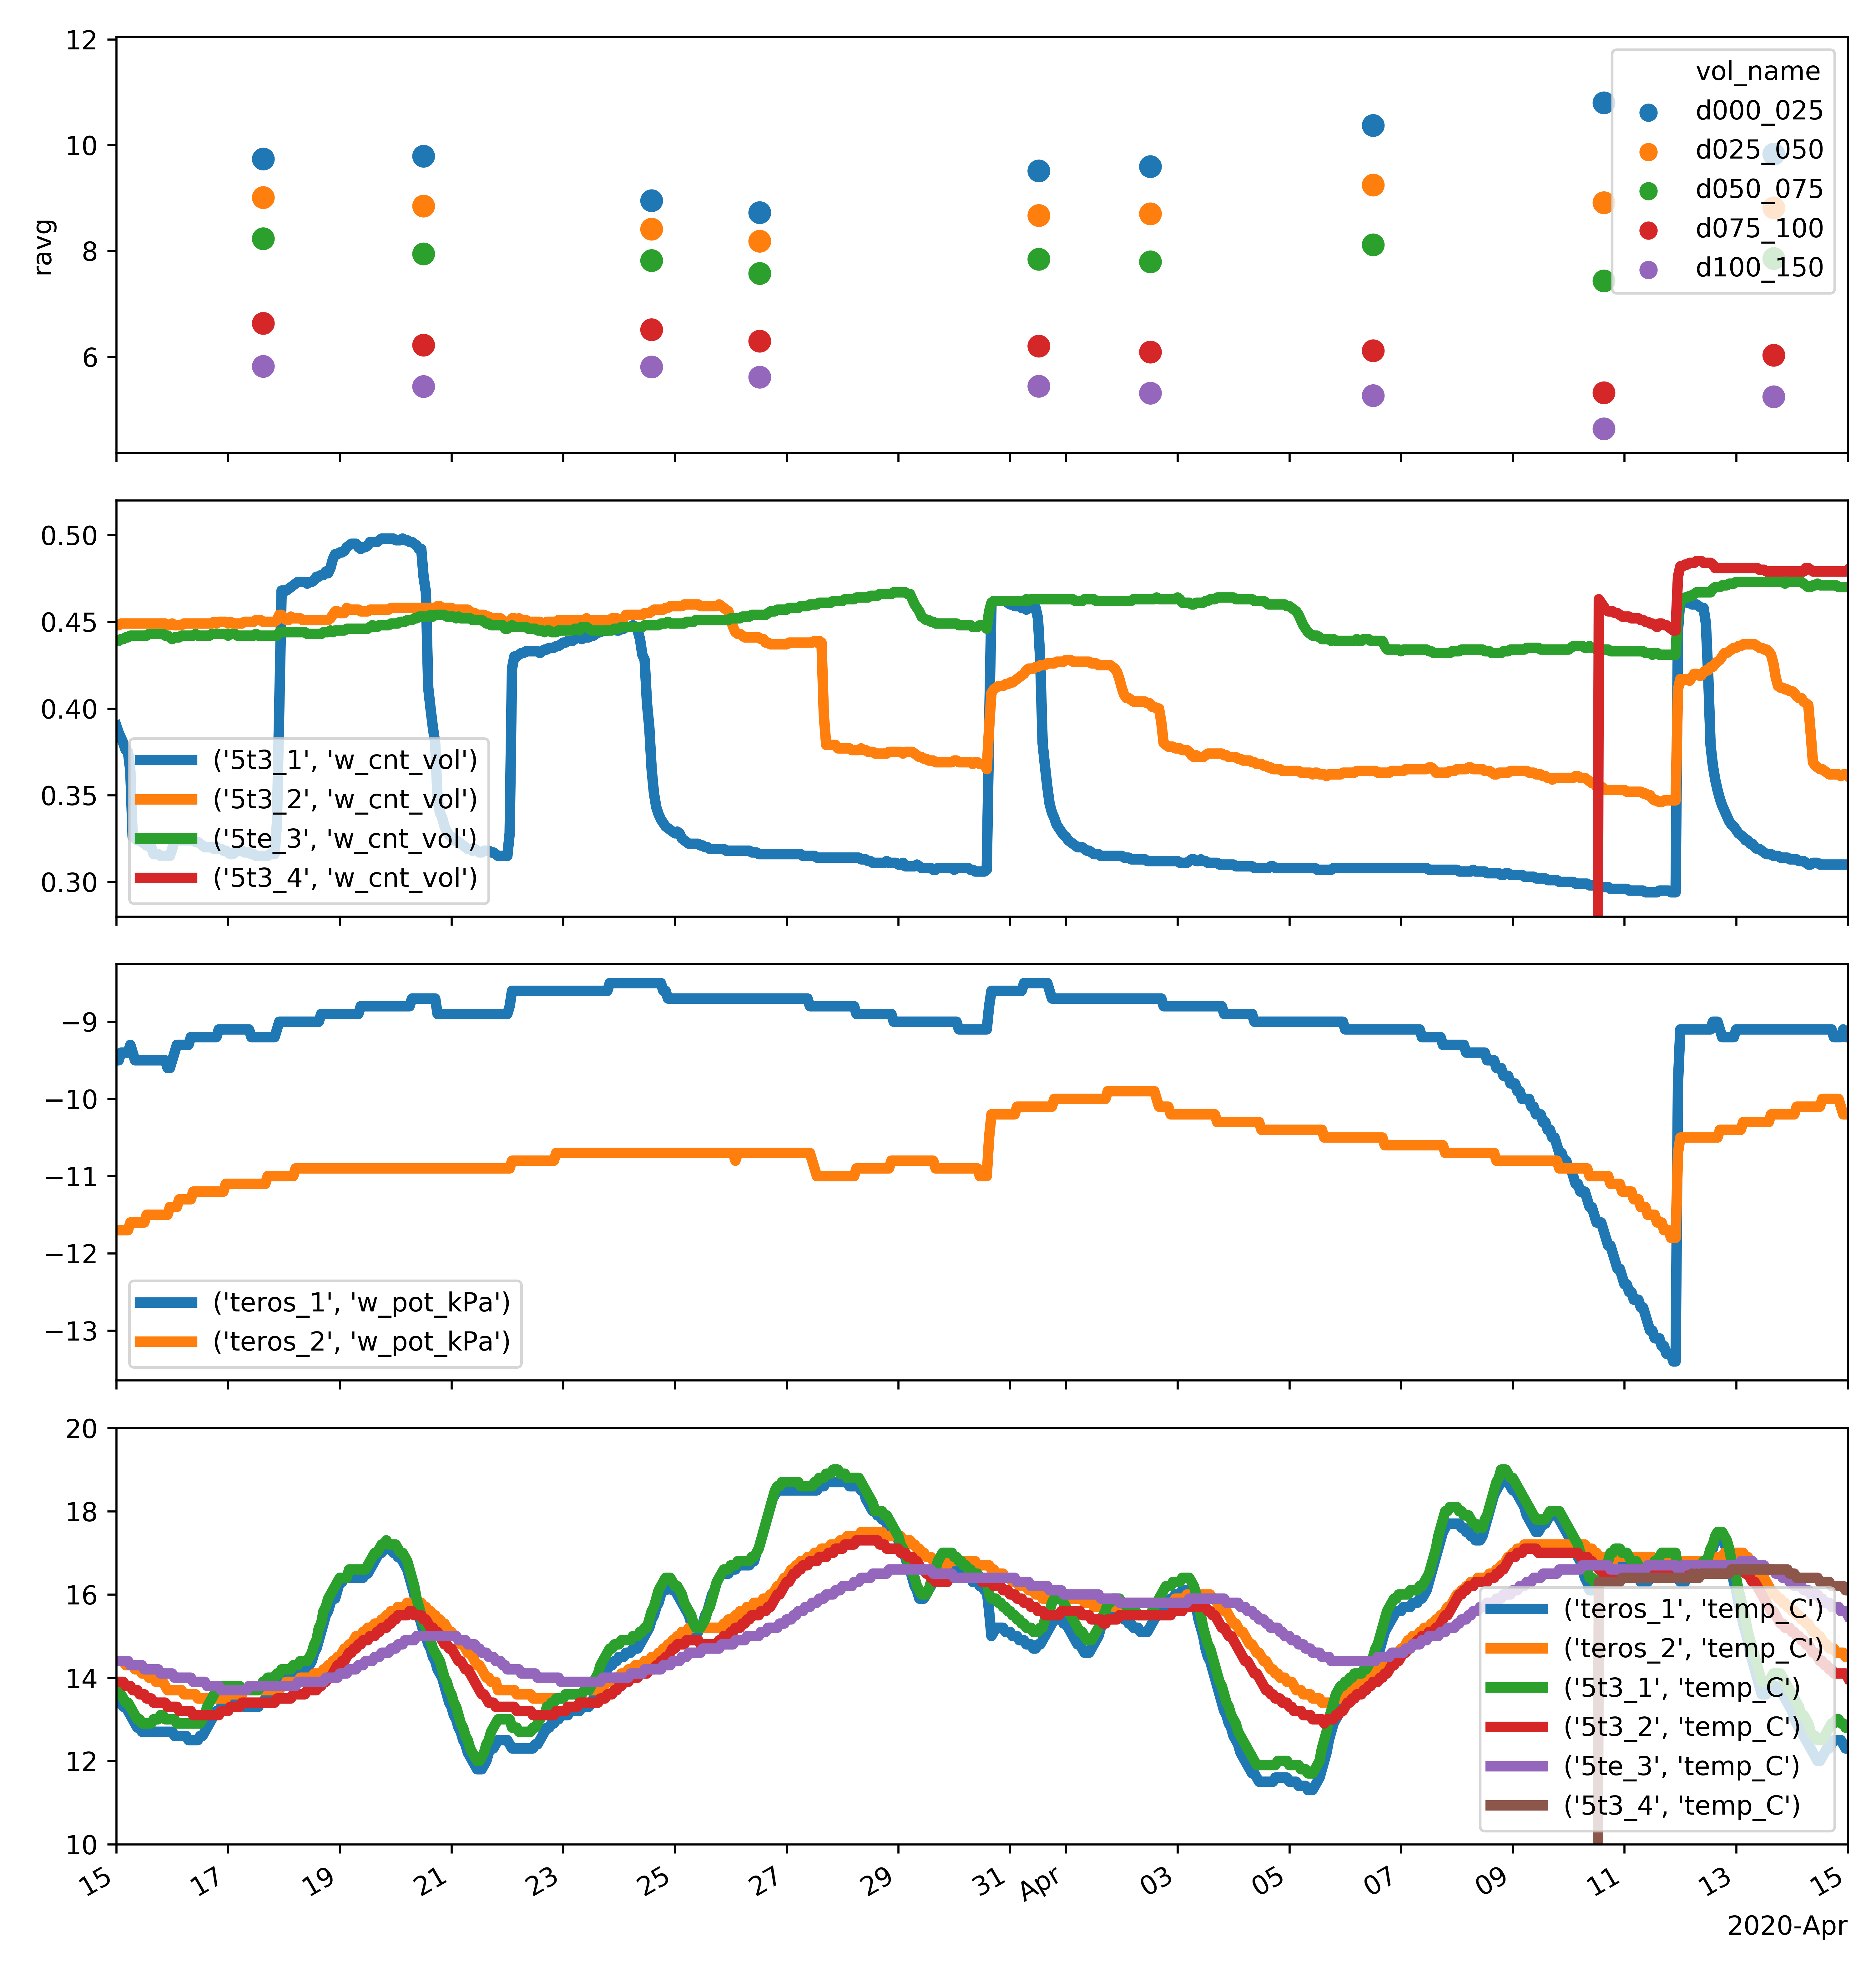
\includegraphics[width=\textwidth]{summary.png}
\end{subfigure}
\caption{Resistivity and soil data.}
\end{figure}

\begin{figure}[H]
\centering
\begin{subfigure}{\textwidth}
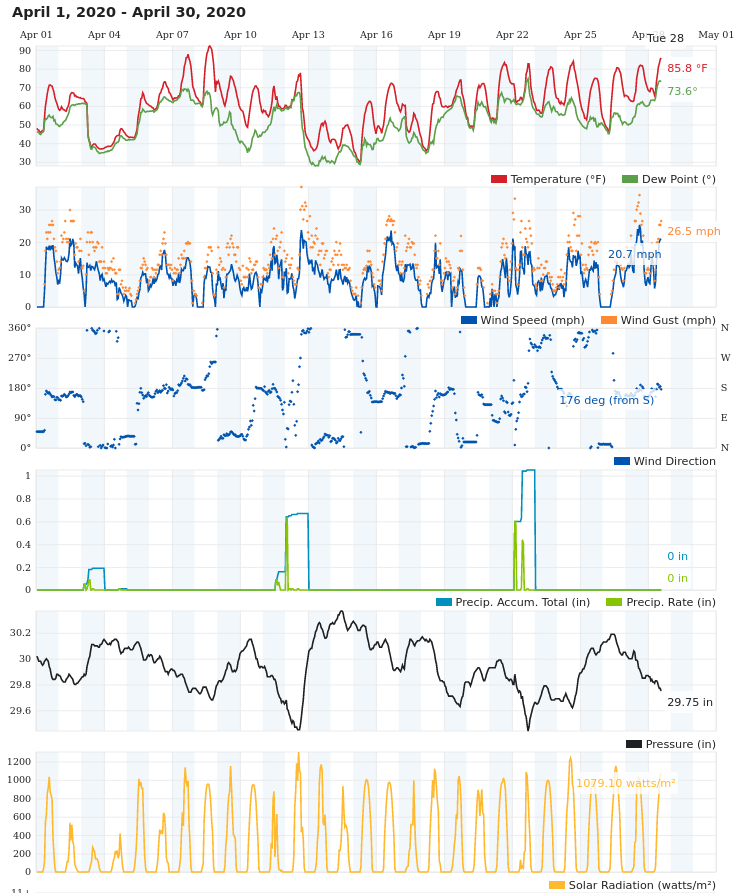
\includegraphics[width=\textwidth]{weatherApril.png}
\end{subfigure}
\end{figure}

\end{document}
